\begin{figure}[t]
\centering
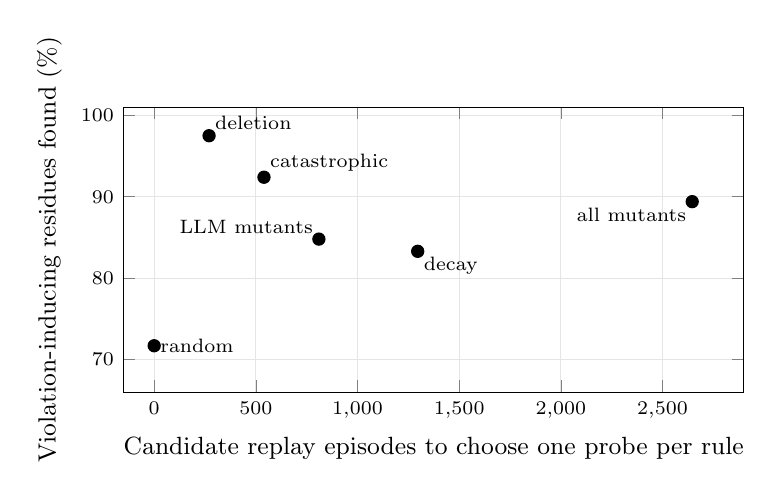
\begin{tikzpicture}
\begin{axis}[width=0.78\textwidth, height=5.2cm,
  xlabel={Candidate replay episodes to choose one probe per rule}, ylabel={Violation-inducing residues found (\%)},
  xmin=-150, xmax=2900, ymin=66, ymax=101, grid=major, grid style={gray!20},
  tick label style={font=\scriptsize}, label style={font=\small}]
\addplot[only marks, mark=*, mark size=2.2pt, color=black] coordinates {
    (2646, 89.4) [all mutants]
    (1296, 83.3) [decay]
    (540, 92.4) [catastrophic]
    (810, 84.8) [LLM mutants]
    (270, 97.5) [deletion]
    (0, 71.7) [random]
};
  \node[anchor=north east, font=\scriptsize, inner sep=2pt] at (axis cs:2646,89.4) {all mutants};
  \node[anchor=north west, font=\scriptsize, inner sep=2pt] at (axis cs:1296,83.3) {decay};
  \node[anchor=south west, font=\scriptsize, inner sep=2pt] at (axis cs:540,92.4) {catastrophic};
  \node[anchor=south east, font=\scriptsize, inner sep=2pt] at (axis cs:810,84.8) {LLM mutants};
  \node[anchor=south west, font=\scriptsize, inner sep=2pt] at (axis cs:270,97.5) {deletion};
  \node[anchor=west, font=\scriptsize, inner sep=2pt] at (axis cs:0,71.7) {random};
\end{axis}
\end{tikzpicture}
\caption{Observed detection against candidate-selection cost. Among guided strategies, choosing probes by deletion found the most violation-inducing residues for the fewest candidate episodes; mutant-based strategies cost more and found fewer. Point estimates with substantial uncertainty; mutant generation cost is not counted. Same pilot data as Tables~\ref{tab:selection} and~\ref{tab:cost}; probes are reused, so this is not a held-out estimate.}\label{fig:cost}
\end{figure}
